\documentclass[twocolumn]{article}
\usepackage[utf8]{inputenc}
\usepackage[top=1.1in, left=0.85in, right=0.85in]{geometry}

% \usepackage{eclbkbox}
\usepackage{amsmath}
\usepackage{amssymb}
\usepackage{code}
\usepackage{url}
% \usepackage{amscd}
% \usepackage{xy}
\usepackage{graphicx}

% \pagestyle{empty}

% \usepackage{ulem}
% go back to italics for emphasis, though
% \normalem

\usepackage{natbib}

\begin{document} 

\title{What, if anything, is epsilon?}
\author{Dr.~Tom~Murphy~VII~Ph.D.\thanks{
Copyright \copyright\ 2013 the Regents of the Wikiplia
Foundation. Appears in SIGBOVIK 2013 with the careless accounting of the
Association for Computational Heresy; {\em IEEEEEE!} press,
Verlag-Verlag volume no.~0x40-2A.
\yen 0.00}
}


\renewcommand\>{$>$}
\newcommand\<{$<$}

\newcommand\CC{{C\nolinebreak[4]\hspace{-.05em}\raisebox{.4ex}{\tiny\bf ++}}}

\date{1 April 2014}

\maketitle

\begin{abstract}
We present a sample of the values of the programming constant {\tt
  epsilon} as found on the internet, for several different programming
languages and with a variety of visualizations.
\end{abstract}

\vspace{1em}
{\noindent \small {\bf Keywords}:
 computational archaeology, epsilon, very-small and medium-small numbers
}

\section*{Introduction}

Epsilon, the all-spelled-out version of $\epsilon$, although properly
``epsilon'' because it's the {\em lowercase} Greek letter, though it's
not like I'm going to start my paper with a lowercase letter even if
it's technically correct, since I like to wait at least until the
second or third letter of the paper before the reader starts doubting
that I can write or spell or have shift-keys on my keyboard, anyway
epsilon is a mathematical symbol denoting a {\em very small number}.

% (intro about math definition in \epsilon--\delta formulation of limits.
% it's not that complicated)

In mathematics, $\epsilon$ usually refers to the
$\epsilon$--$\delta$ formulation of limits. This is pretty simple and a
reminder appears in Figure~\ref{fig:epsilondelta}. This paper is not
about that kind of math.

In computing, $\epsilon$ is used in a much more general sense to just
mean some small number or error bound. For example, two numbers are
often considered equal if their absolute difference is less than
$\epsilon$.

In IEEE-754 floating-point~\cite{ieee754}, the standard way that
computers represent ``real numbers,'' there is a specific formal value
called ``machine epsilon'', or ``unit roundoff''. It is the maximum
(relative) amount of error from a single rounding operation. This
number is useful if you want to do numerical programming and be
careful about what you're doing.

Most programmers find this subject too tedious and simply pick a
number that seems pretty small. Thus in practice, $\epsilon$ is an
application-specific choice. Of well-known ``constants,'' $\epsilon$
may be the least agreed-upon, with values seen in the wild spanning
more than {\em 300 orders of magnitude}. This paper explores the
practical values of $\epsilon$ in real software.

\begin{figure}[ht]
\begin{center}
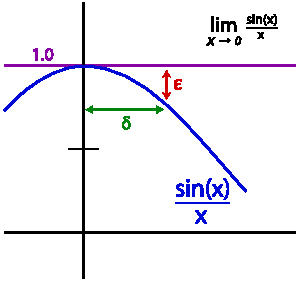
\includegraphics[width=0.90 \linewidth]{epsilondelta.pdf}
\end{center}\vspace{-0.1in}
\caption{ The curvy line is the function $\frac{\sin x}{x}$, which is
  undefined at $0$. However, its limit as $x$ approaches $0$ is $1$.
  The $\epsilon$--$\delta$ formulation of the limit is this: For any
  positive choice of $\epsilon$, there exists some $\delta$ such that
  $\frac{\sin (0 + \delta)}{0 + \delta}$ is less than $1 + \epsilon$.
  In other words, for an arbirarily small error (your choice), I
  can produce a delta from $0$ (my choice) that brings the result
  within the error of the limit. This has nothing to do with the
  subject of the paper.}
\label{fig:epsilondelta}
\end{figure}

\section{Methodology}

\paragraph{Github.} Github is the hub that contains all gits, approximately
10~million of them, as of the beginning of 2014. The site has search
functionality, which ``allowed'' me to scrape one hundred pages of
results for queries like {\tt "const double epsilon ="} for various
languages, as long as I didn't do it too fast. I scraped the
programming languages C, \CC, C$\sharp$, JavaScript, and Objective~C.
Each language has its own idiosyncracies about how constants are
defined, so I used one (or several) appropriate to each language. For
example, in JavaScript, I looked for {\tt "var epsilon ="}. From these
HTML files I extracted all of the right-hand-side expressions,
manually excluded the ones that could not be evaluated (for example
because they depended on other symbols; see
Figure~\ref{fig:cdoubleuninterpretable} for some examples), and then
computed the actual values for the rest. The source code to do the
scraping, extract the expressions, and tally the results is available
online.\!\footnote{In the Subversion repository at:
  \url{https://sourceforge.net/p/tom7misc/svn/HEAD/tree/trunk/epsilon/}}

\begin{figure}[ht]
\begin{center}
\begin{tabular}{l}
\verb+0.5/ELEC_REST_ENERGY+ \\
\verb+alpha/beta+ \\
\verb+4 / MULT32+ \\
\verb+exact_epsilon(true)+ \\
\verb+fmass_Epsilon * EPS_EXTRA+ \\
\verb+((Lj_Parameters*) parameters)->+ \\
\verb+scalar_traits<+ \\
\verb+EpsArray[prec]+ \\
\verb+hfwfn_->+ \\
\verb+fl.net_.opt_.epsilon+ \\
\verb+Tolerance+ \\
\end{tabular}
\end{center}\vspace{-0.1in}
\caption{ Other uninterpretable values of {\tt const double epsilon}
  in C. Who knows what these are supposed to be?}
\label{fig:cdoubleuninterpretable}
\end{figure}

\paragraph{SPEC benchmarks.} Did you know that the SPEC 
benchmarks~\cite{spec2006} cost \$800? Like they literally expect me
to pay them money to download the source code so that I could grep for
{\tt const double epsilon} or test my compiler out on that. Many are
even based on open-source software like Sphinx and POV-Ray.
Ridiculous. I refuse. Values of epsilon for the SPEC benchmarks do not
appear in Figure~\ref{fig:spec}.

\begin{figure}[ht]
\begin{center}

\includegraphics[width=0.99 \linewidth]{spec.pdf}
\end{center}\vspace{-0.1in}
\caption{\$800? Fuck that!}
\label{fig:spec}
\end{figure}

\section{Results}

The results of the analysis appear in several figures which are
interspersed haphazardly with this text. Each figure presents the data
in a different way, since this diversity in presentation should
maximize the chance that one of the charts makes sense to you. The C
programming language has two numeric types that could reasonably be
used to represent $\epsilon$: {\tt float} and {\tt double}. The
results for {\tt double} appear in Figure~\ref{fig:cdouble} and for
{\tt float} in Figure~\ref{fig:cfloat}. \CC\ has those same two types,
but I decided arbitrarily to only look at {\tt double}, which is in
Figure~\ref{fig:cppdouble}. Programmers in C$\sharp$ are very
creative; their results are presented in Figure~\ref{fig:csharp}.
Objective~C proved unpopular for use of $\epsilon$, its sparse data
are in Figure~\ref{fig:objectivec}. Finally, the ineffable JavaScript
has its results in Figure~\ref{fig:javascript}.

\begin{figure}[ht]
\begin{center}
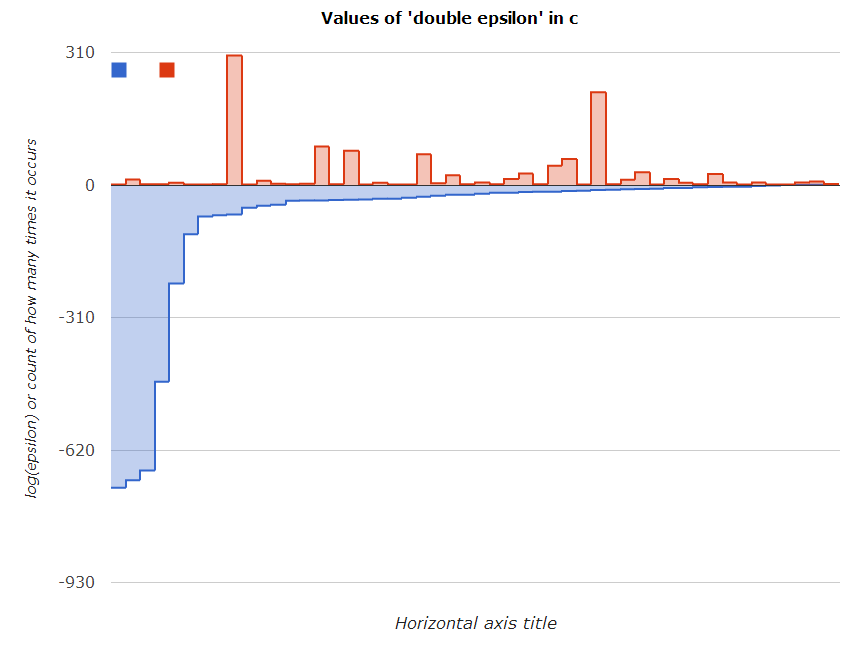
\includegraphics[width=0.99 \linewidth]{chart-c-double}
\end{center}\vspace{-0.1in}
\caption{ Values for {\tt const double epsilon} in the C programming
  language. In this chart, the blue (lower) bars are the distinct values
  of epsilon seen. The vertically aligned red (upper) bar is its count.
  Epsilon values are plotted on a logarithmic scale, where the minimum
  observed value $\log(-708)$ is $303 \times 10^{-308}$, and the largest
  $\log(1.609)$ is $5$. 
  %
  Notes: One programmer used the value {\tt -1e10}, which is
  -10,000,000,000, probably meaning {\tt 1e-10}. This value was excluded
  because it has no real logarithm.
}
\label{fig:cdouble}
\end{figure}

\begin{figure}[ht]
\begin{center}
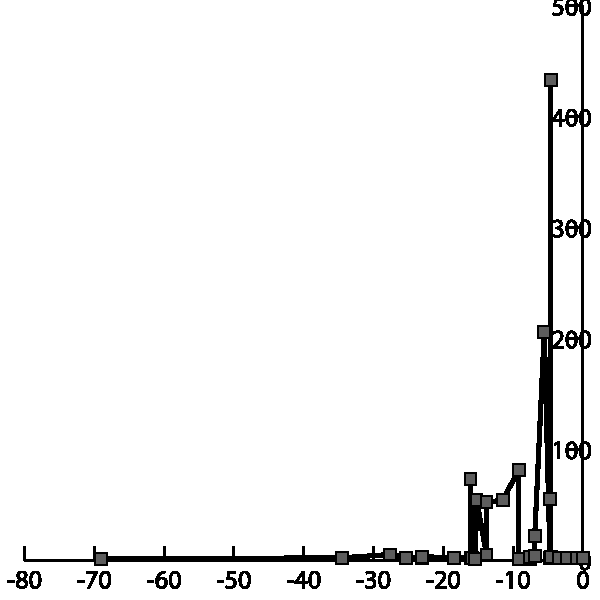
\includegraphics[width=0.99 \linewidth]{chart-c-float}
\end{center}\vspace{-0.1in}
\caption{ Values for {\tt const float epsilon} in the C programming
  language. An $x$--$y$ scatter plot where the $y$ coordinate is the
  count of the number of times that specific value occurred, and the
  $x$ coordinate is the log of the value. Values take on a less
  extreme range than with type {\tt double}, naturally, ranging ``only''
  31 orders of magnitude from $3.9 \times 10^{-31}$ to $0$.}
\label{fig:cfloat}
\end{figure}


\begin{figure}[ht]
\begin{center}
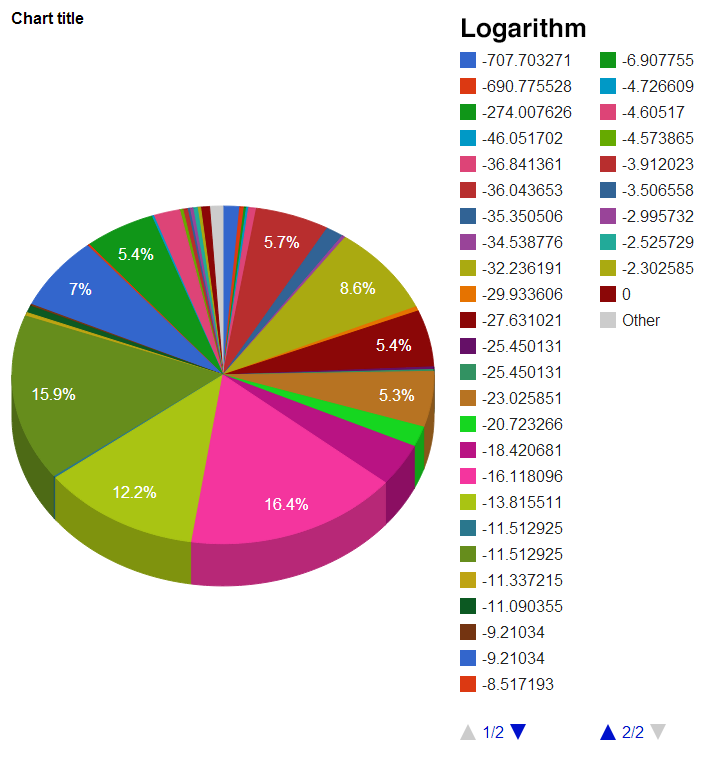
\includegraphics[width=0.99 \linewidth]{chart-cpp}
\end{center}\vspace{-0.1in}
\caption{
  Values for {\tt const double epsilon} and {\tt constexpr
    double epsilon} in the C++ programming language. The {\tt
    constexpr} qualifier, a new feature of C++11, is used very rarely
  (less than 1\% of the time).
  %
  Notes:
  Five times, the programmer used 0.0 for epsilon, which is possibly
  the only unjustifiable value. The value {\tt pow(10,-13)} is
  annotated in German ``Genauigkeitsziel bei der Nullstellensuche,''
  or ``Accuracy goal in the search for zeros.'' }
\label{fig:cppdouble}
\end{figure}

\begin{figure}[ht]
\begin{center}
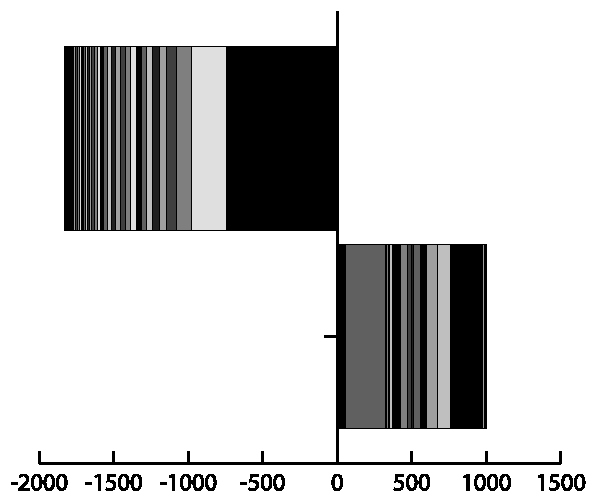
\includegraphics[width=0.99 \linewidth]{chart-csharp}
\end{center}\vspace{-0.1in}
\caption{ Values for {\tt const double epsilon} in the C$\sharp$
  programming language. In this chart, the left edge of greyscale
  blocks on the left-facing flag represent the cumulative value of the
  logarithm of all values of epsilon seen so far. The right edge of
  the block with the exact same greyscale value on the bottom-right
  flag is the cumulative count of all definitions of epsilon so far.
  It is easy to see that there are 1,000 total definitions, as
  expected.
  %
  Notes: One programmer defined epsilon as {\tt 1.0-18}, that is,
  -17, probably meaning {\tt 1.0e-18}. Four used literal {\tt 0} for
  epsilon. Another defined epsilon as {\tt 1 / 100000}, which uses
  integer division and results again in 0. Owing to the strength and
  creativity of C$\sharp$ developers, here we saw our largest
  value of epsilon so far, {\tt 700}, and the declaration with the most
  significant digits: {\tt
    0.0000000000000002220446049250313080847263336181640625}.
}
\label{fig:csharp}
\end{figure}

\begin{figure}[ht]
\begin{center}
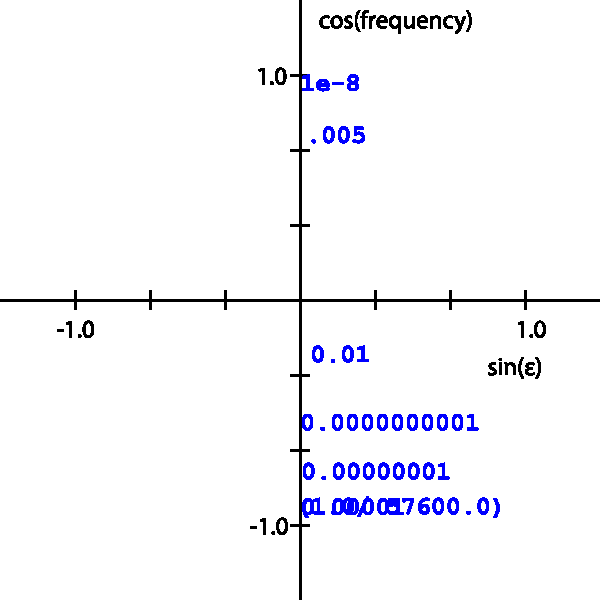
\includegraphics[width=0.99 \linewidth]{chart-objectivec}
\end{center}\vspace{-0.1in}
\caption{Results for the language Objective~C for {\tt const double epsilon}.
Perhaps because Objective~C programmers do not use this idiom for defining
constants, or because it is only used to make iPhone games where epsilon is
not a concept of interest, there were only 8 distinct values of epsilon
observed. This allows us to present the data completely in the chart. The
$x$ axis is $\sin(\epsilon)$ and the $y$ axis is $\cos(f)$ where $f$ is
the total number of times that the given value occurred in the code.}
\label{fig:objectivec}
\end{figure}

\begin{figure}[ht]
\begin{center}
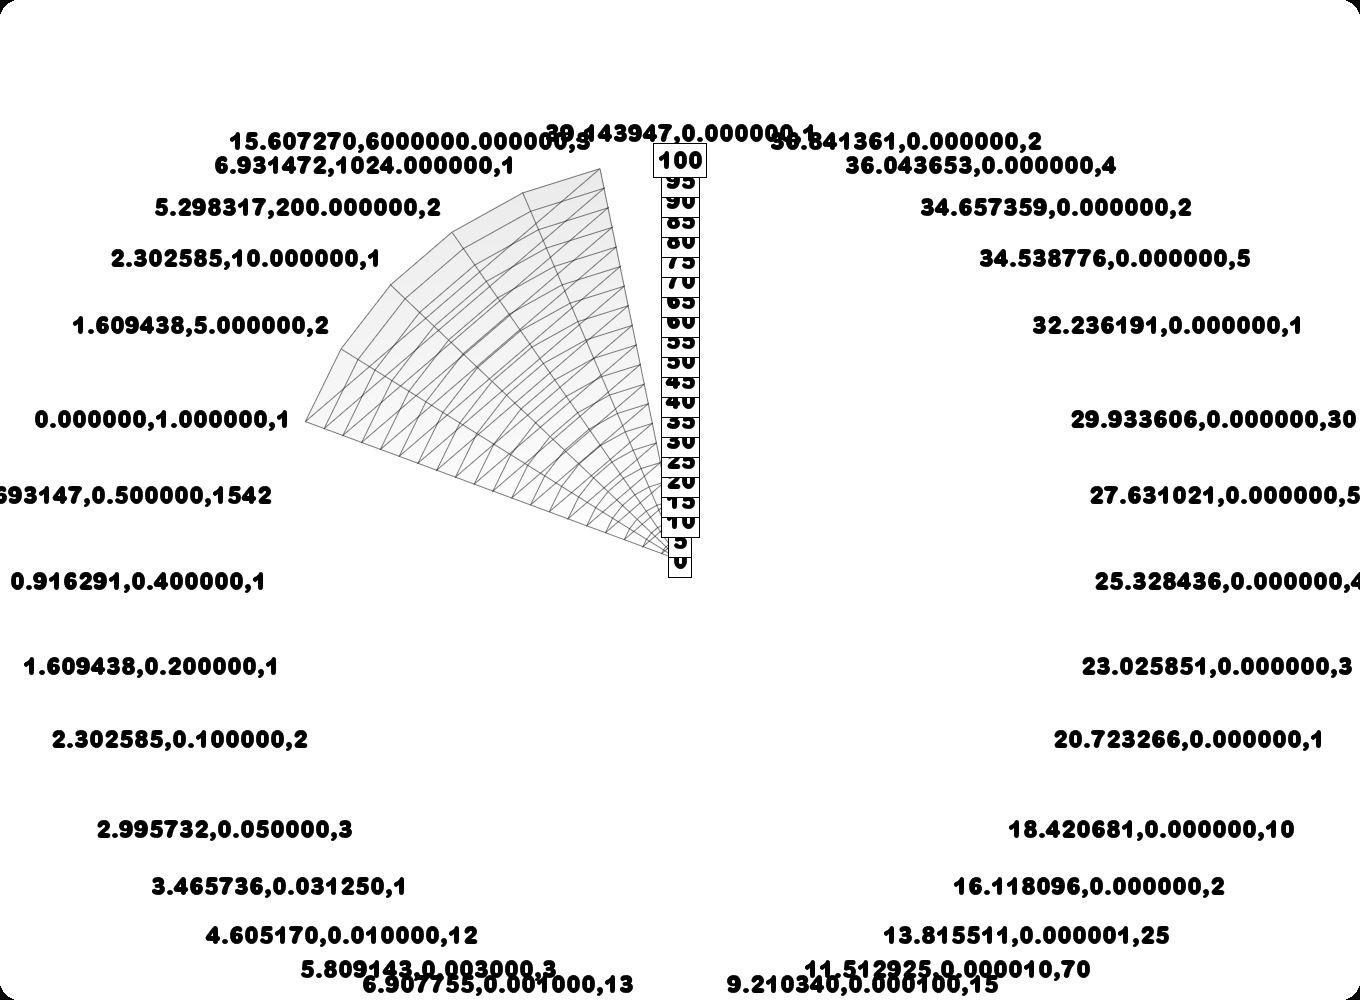
\includegraphics[width=0.70 \linewidth]{chart-js}
\end{center}\vspace{-0.1in}
\caption{Finally, JavaScript, the official language of the Internet.
  In this ``radar'' plot, the data are arranged around a circle, as
  tuples of $\langle \log(\epsilon), \epsilon, f \rangle$ where $f$ is
  the frequency of the value being observed. Numbers in boxes ascend
  along the $0\deg$ axis, displaying each of the multiples of 5
  between 0 and 100, inclusive. Boxes stack so that only part of the
  number is visible, but you know what's under there if you've looked
  at numbers before. A spider-web-like network of interlacing lines
  ascribe some additional meaning to some of the points on the clock
  face. The smallest nonzero value observed was $10^{-32}$.
%
  Notes: JavaScript programmers have the highest tolerance for error
  of all languages tested, with over 1,000 using epsilon of 0.5 or
  higher. One programmer used $\epsilon = 1024$, and another
  6,000,000! }
\label{fig:javascript}
\end{figure}


\bibliography{paper}{}
\bibliographystyle{plain}
\end{document}
